%---------------------------------------------------------------------
%	个性化信息
%--------------------------------------------------------------------
\newcommand{\MYTITLE}{}%论文标题
\newcommand{\MYID}{2022310210}%学号
\newcommand{\MYNAME}{陆知雨}%姓名
\newcommand{\MYCLASS}{财政学(财政基础理论)22}%班级
\newcommand{\MYADVISOR}{}%任课教师
\newcommand{\MYCOURSE}{}%课程名
\newcommand{\MYTERM}{2023年春季学期}%学期
\newcommand{\MYCOURSEID}{}%课程ID
%---------------------------------------------------------------------
%   各种导言
%--------------------------------------------------------------------
\documentclass[a4paper,12pt]{report}
\usepackage{geometry} % to change the page dimensions
\geometry{a4paper,left=2.5cm,right=2.5cm,top=2.54cm,bottom=2.54cm}%页边距
\usepackage{ctex}
\usepackage{xeCJK}
\usepackage{comment}
\usepackage{setspace}
\usepackage{fancyhdr}
\usepackage{graphicx}
\usepackage{wrapfig}
\usepackage{subfigure}
\usepackage{array}
\usepackage{titlesec}
\usepackage{titletoc}
\usepackage[titletoc]{appendix}
%\usepackage[top=30mm,bottom=30mm,left=20mm,right=20mm]{geometry}
%\usepackage{cite}

%\usepackage{courier}
\setmonofont{Courier New}
\usepackage{listings}
%---------------------------------------------------------------------
%   参考文献设置 
%   论文引用示例\cite{ }
%--------------------------------------------------------------------
\usepackage{natbib}
\bibliographystyle{plain}
%---------------------------------------------------------------------
%	引用文献设置为上标
%---------------------------------------------------------------------
\begin{comment}
    \makeatletter
    \def\@cite#1#2{\textsuperscript{[{#1\if@tempswa , #2\fi}]}}
    \makeatother
\end{comment}

\lstset{tabsize=4, keepspaces=true,
    xleftmargin=2em,xrightmargin=0em, aboveskip=0.1em,
    %backgroundcolor=\color{gray!20},  % 定义背景颜色
    frame=none,                       % 表示不要边框
    extendedchars=false,              % 解决代码跨页时,章节标题,页眉等汉字不显示的问题
    numberstyle=\ttfamily,
    basicstyle=\ttfamily,
    keywordstyle=\color{blue}\bfseries,
    breakindent=10pt,
    identifierstyle=,                 % nothing happens
    commentstyle=\color{green}\small,  % 注释的设置
    morecomment=[l][\color{green}]{\#},
    numbers=left,stepnumber=1,numberstyle=\scriptsize,
    showstringspaces=false,
    showspaces=false,
    flexiblecolumns=true,
    breaklines=true, breakautoindent=true,breakindent=4em,
    escapeinside={/*@}{@*/},
}
\usepackage{amsmath}
\usepackage{amsthm}
\newtheorem{theorem}{定理}
\newtheorem{definition}{定义}
\newtheorem{corollary}{推论}
\newtheorem{example}{例}
\renewcommand {\thetable} {\arabic{table}}
\renewcommand {\thefigure} {\arabic{figure}}
\usepackage{amsfonts}
\usepackage{lipsum}
%\usepackage{bm}
\usepackage{booktabs} % for much better looking tables
\usepackage{paralist} % very flexible & customisable lists (eg. enumerate/itemize, etc.)
\usepackage{verbatim} % adds environment for commenting out blocks of text & for better verbatim
\usepackage{subfigure} % make it possible to include more than one captioned figure/table in a single float
% These packages are all incorporated in the memoir class to one degree or another...
\usepackage{cases} %equation set
\usepackage{multirow} %use table
\usepackage{algorithm}
\usepackage{algorithmic}
%\usepackage{cite}
\usepackage{hyperref}
\usepackage{longtable}
\usepackage{caption}
\usepackage{zhnumber} % change section number to chinese
\hypersetup{colorlinks,linkcolor=black,anchorcolor=black,citecolor=black, pdfstartview=FitH,bookmarksnumbered=true,bookmarksopen=true,} % set href in tex & pdf
%\usepackage[framed,numbered,autolinebreaks,useliterate]{mcode} % 插入matlab代码
\XeTeXlinebreaklocale "zh"
\XeTeXlinebreakskip = 0pt plus 1pt minus 0.1pt
\setlength{\baselineskip}{22pt}
%---------------------------------------------------------------------
%	图表顺序标号,不分章节
%---------------------------------------------------------------------
\usepackage{chngcntr}
\counterwithout{table}{chapter}
\counterwithout{table}{section}
\counterwithout{figure}{chapter}
\counterwithout{figure}{section}
\counterwithout{equation}{chapter}
\counterwithout{equation}{section}


\titleclass{\chapter}{straight}%禁止chapter换页
%---------------------------------------------------------------------
%	页眉页脚设置
%---------------------------------------------------------------------
\fancypagestyle{plain}{
    \pagestyle{fancy}      %改变章节首页页眉
}

\pagestyle{fancy}
\lhead{}
\rhead{}
\fancyhead[C]{\MYTITLE}
\cfoot{\thepage}
\renewcommand\thesection{(\zhnum{section})}
\renewcommand \thesubsection {\arabic{subsection}.}
\renewcommand \thechapter {\zhnum{chapter}、}
\titleformat{\chapter}{\centering\zihao{4}\songti\bfseries}{\chinese{chapter}、}{0.05em}{}
\titlespacing{\chapter}{12pt}{12pt}{*3}
\titlespacing{\section}{0pt}{0pt}{*0}
\titlespacing{\subsection}{0pt}{0pt}{*0}
\titleformat{\section}{\zihao{-4}\songti\bfseries}{$\qquad$(\chinese{section})}{0.05em}{}
\titleformat{\subsection}{\zihao{-4}\songti\mdseries}{$\qquad$\arabic{subsection}.$\ $}{0.05em}{}

%---------------------------------------------------------------------
%	摘要设置
%---------------------------------------------------------------------
%\renewcommand{\abstractname}{摘要}
\newcommand{\enabstractname}{ABSTRACT}
\newcommand{\cnabstractname}{内容摘要}
\newenvironment{enabstract}{%
  \par\small
  \noindent\mbox{}\hfill{\bfseries \zihao{3} \enabstractname}\hfill\mbox{}\par
  \vskip 2.0ex}{\par\vskip 2.0ex}
\newenvironment{cnabstract}{%
  \par\small
  \noindent\mbox{}\hfill{\bfseries \zihao{3} \cnabstractname}\hfill\mbox{}\par
  \vskip 2.0ex}{\par\vskip 2.0ex}
\renewcommand{\figurename}{图}
\renewcommand{\tablename}{表}
%---------------------------------------------------------------------
%	目录页设置
%---------------------------------------------------------------------
%\renewcommand{\contentsname}{\zihao{-3} 目\quad 录}
\setcounter{tocdepth}{1}
\renewcommand{\contentsname}{\zihao{3}\bfseries\centering{目$\quad$录}}
\titlecontents{chapter}[0em]{\songti\zihao{4}\bfseries}{\thecontentslabel\ }{}
{\hspace{.5em}\titlerule*[4pt]{$\cdot$}\contentspage}
\titlecontents{section}[2em]{\vspace{0.1\baselineskip}\songti\zihao{4}}{\thecontentslabel\ }{}
{\hspace{.5em}\titlerule*[4pt]{$\cdot$}\contentspage}
%\titlecontents{subsection}[4em]{\vspace{0.1\baselineskip}\songti\zihao{-4}}{\thecontentslabel\ }{}
%{\hspace{.5em}\titlerule*[4pt]{$\cdot$}\contentspage}
\begin{document}
%---------------------------------------------------------------------% 
%	封面设置
%---------------------------------------------------------------------
\begin{titlepage}
    \begin{center}

        
\includegraphics[width=1.0\textwidth]{figure/zhongcai.png}\\
        \vspace{20mm}
        \textbf{\zihao{2}{\heiti\textbf{\MYTITLE}}}\\[0.8cm]
        \vspace{10mm}
        \vspace{\fill}

        \setlength{\extrarowheight}{3mm}
        {\songti\zihao{3}
            \begin{tabular}{rp{8cm}<{\centering}}
                {\makebox[4\ccwd][s]{学年学期:}}       & \kaishu \underline{\makebox[8cm]{\MYTERM}}     \\
                {\makebox[4\ccwd][s]{课程名称:}}       & \kaishu \underline{\makebox[8cm]{\MYCOURSE}}   \\
                {\makebox[4\ccwd][s]{课程代码:}}       & \kaishu \underline{\makebox[8cm]{\MYCOURSEID}} \\
                {\makebox[4\ccwd][s]{任课教师:}}       & \kaishu \underline{\makebox[8cm]{\MYADVISOR}}  \\
                {\makebox[4\ccwd][s]{班\qquad 级:}}    & \kaishu \underline{\makebox[8cm]{\MYCLASS}}    \\
                {\makebox[4\ccwd][s]{学\qquad 号:}}    & \kaishu \underline{\makebox[8cm]{\MYID}}       \\
                {\makebox[4\ccwd][s]{姓\qquad 名:}}    & \kaishu \underline{\makebox[8cm]{\MYNAME}}     \\
                \\
                {\makebox[4\ccwd][s]{总\qquad 分:}}    & \kaishu \underline{\makebox[8cm]{}}            \\
                {\makebox[4\ccwd][s]{评$\ $分$\ $人:}} & \kaishu \underline{\makebox[8cm]{}}            \\
            \end{tabular}
        }\\[2cm]
    \end{center}
\end{titlepage}

%---------------------------------------------------------------------
%  摘要页
%---------------------------------------------------------------------
\setcounter{page}{1}
\begin{cnabstract}
%此处输入摘要内容

    \par\textbf{关键字: } 关键字1,关键字2,关键字3
\end{cnabstract}

\begin{enabstract}
%此处输入英文摘要内容

    \par\textbf{KEY WORDS:} keyword1, keyword2, keyword3
\end{enabstract}
%\thispagestyle{empty}
\newpage

%---------------------------------------------------------------------
%  目录页
%---------------------------------------------------------------------
\setcounter{page}{1}
\tableofcontents % 生成目录
%\thispagestyle{empty}
\newpage
%---------------------------------------------------------------------
%  引言
%---------------------------------------------------------------------

\chapter*{\zihao{3} \heiti \MYTITLE}
\setcounter{page}{1}
%这里写引言

%---------------------------------------------------------------------
%  正文
%---------------------------------------------------------------------
\chapter{章节标题示例}
\section{二级标题示例}
\subsection{三级标题示例}
%表格例
\begin{table}[h]
    \centering
    \begin{tabular}{lc}
        \toprule[1.5pt]
        成员       & 分工                                        \\
        \midrule[1.0pt]
        博丽灵梦   & 组长、初期报告展示、复制报告汇总            \\
        雾雨魔理沙 & 稳健OLS与FGLS回归估计及分地区、年度差异分析 \\
        东风谷早苗 & 分位数回归、分地区回归、年度差异分析        \\
        十六夜宵夜 & 数据处理、期末汇报展示                      \\
        魂魄妖梦   & 数据处理、中期报告展示、排版整理            \\
        \bottomrule[1.5pt]
    \end{tabular}
\end{table}


%拆行公式例:
\begin{equation}
    \begin{split}
        UNEMSEC = \beta_0 + \beta_1HEA\_0 + \beta_2HEA\_1 + \beta_3OLD\_0 +  \\
        \beta_4OLD\_1 + \beta_5ifiwork + \beta_6family\_income + \epsilon
    \end{split}
%引用例子
\begin{quotation}

\end{quotation}


%插入图片及添加图片脚注示例
\begin{figure}[H]
    \centering
    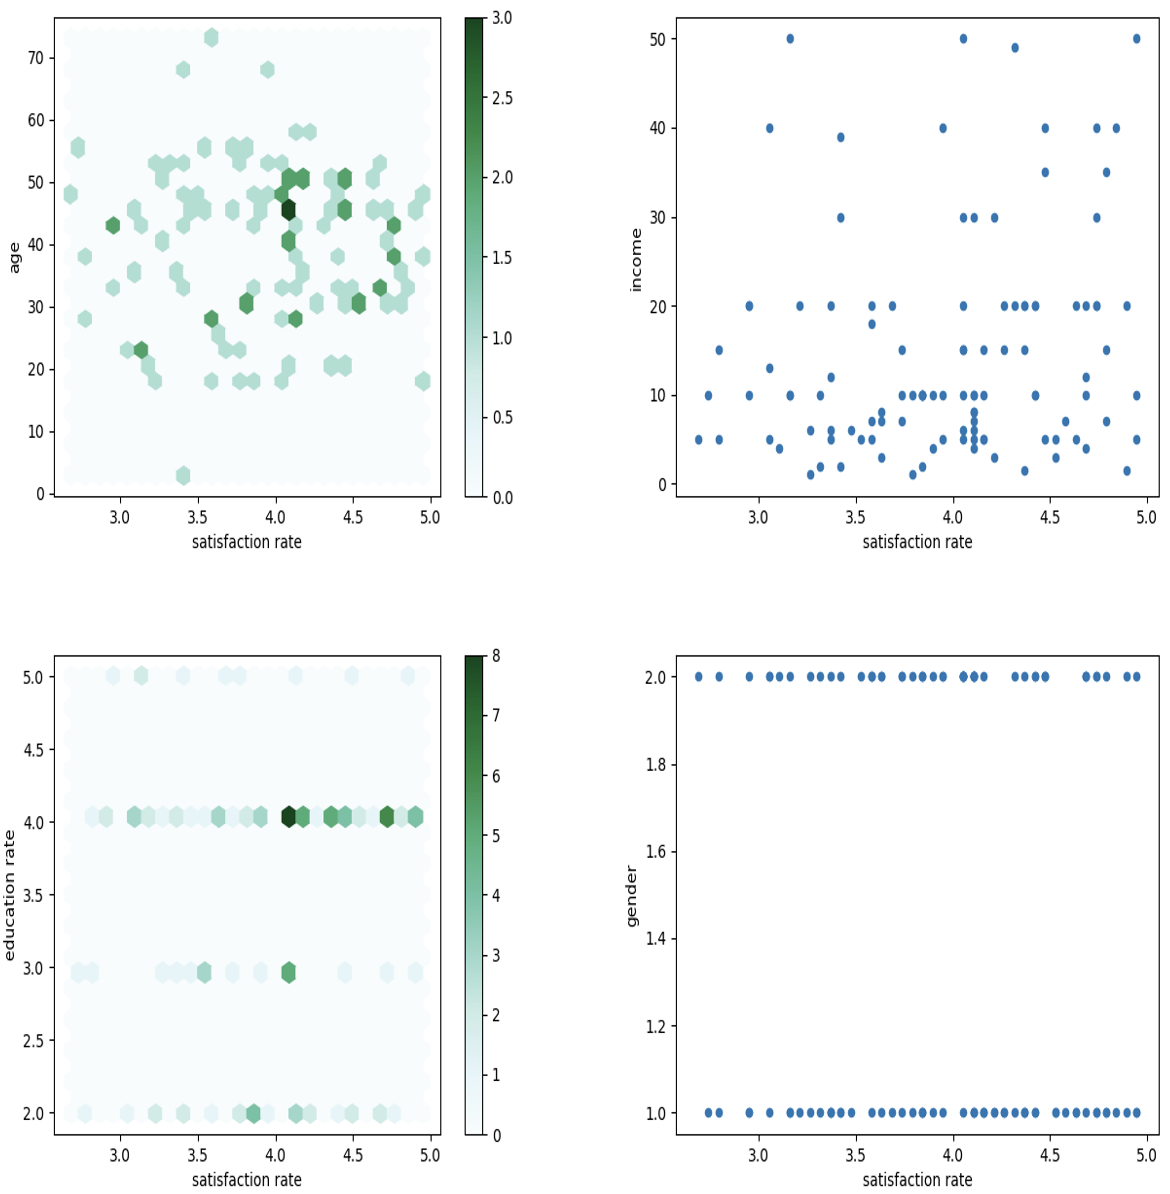
\includegraphics[width=0.85\textwidth]{figure/table1.png}
    \caption{满意指数与关于年龄、家庭人均收入、受教育程度、性别关系 \protect\footnotemark[1]}
\end{figure}
 \footnotetext[1]{
Satisfaction rate(满意指数):为人们对于市域社会治理的九个方面的满意评分求均值,范围(1-5分)
 
 Age(年龄):指填表者年龄

 Income(收入):指家庭人均年收入 (单位:万元)

 Education rate(受教育程度):通过1至5的递增的数值代表小学及以下,初中/高中/中专,大专,本科,硕士及以上五种最高学历

 Gender(性别):1——男性,2——女性
}



%插入代码示例:
\begin{lstlisting}[language=C]
    qui reg SR1 $xx dummy1-dummy24 if time==0
    predict e1,res
    g e2 = e1^2
    g lne2 = log(e2)
    qui reg lne2 peincome if time==0,noc
    predict lne2f
    g e2f =exp(lne2f)
    reg SR1 $xx dummy1-dummy24 if time==0 [aw=1/e2f]
\end{lstlisting}


%---------------------------------------------------------------------
%  参考文献
%---------------------------------------------------------------------

\bibliography{此处输入bib文件名}

\end{document}
